% !TEX program = tectonic
%
% EMNLP 2026 submission draft.
% Compile:
%   ~/bin/tectonic paper.tex
%
% Note: this draft uses a self-contained article-class layout that mimics the
% EMNLP/ACL look (11pt, two-column, single-spaced). For the final submission,
% drop acl.sty from https://github.com/acl-org/acl-style-files into this
% directory and replace the preamble with `\documentclass[11pt]{article}\usepackage{acl}`.

\documentclass[11pt,a4paper]{article}

\usepackage[T1]{fontenc}
\usepackage[utf8]{inputenc}
\usepackage{times}
\usepackage{microtype}

\usepackage[a4paper,
            top=2.5cm, bottom=2.5cm,
            left=2cm, right=2cm,
            columnsep=0.7cm]{geometry}

\usepackage[hidelinks]{hyperref}
\usepackage{url}
\usepackage{graphicx}
\graphicspath{{../figures/}}
\usepackage{amsmath,amssymb}
\usepackage{booktabs}
\usepackage{multirow}
\usepackage{xcolor}
\usepackage{natbib}
\bibliographystyle{plainnat}

% ACL-like section spacing
\usepackage{titlesec}
\titlespacing*{\section}{0pt}{1.6ex}{0.8ex}
\titlespacing*{\subsection}{0pt}{1.2ex}{0.6ex}

% Shared math notation for the paper.
\newcommand{\R}{\mathbb{R}}
\newcommand{\E}{\mathbb{E}}
\newcommand{\Df}{\mathcal{D}_f}
\newcommand{\Dr}{\mathcal{D}_r}
\newcommand{\PPL}{\mathrm{PPL}}
\newcommand{\Lone}{L_1}
\newcommand{\Ltwo}{L_2}
\newcommand{\Lthree}{L_3}
\newcommand{\Lforget}{L_F}
\newcommand{\Lneigh}{L_N}
\newcommand{\Lbyst}{L_B}
\DeclareMathOperator*{\argmin}{arg\,min}
\DeclareMathOperator*{\argmax}{arg\,max}
\newcommand{\geomean}{\mathrm{geo}}

\title{From Three-Layer Unlearning Impact to Forget-Set Audit:\\
       Predicting Impact Profiles from Forget-Set Geometry Alone}

\author{Anonymous EMNLP submission}
\date{}

\begin{document}
\twocolumn[
  \maketitle
  \begin{@twocolumnfalse}
    % Abstract structure: problem, gap, method, key mechanism, results, claim.
    \begin{abstract}
      % Problem.
      Large language model (LLM) unlearning must remove target knowledge represented by a forget set $\Df$ while limiting collateral damage to useful knowledge.
      % Gap.
      Existing evaluations usually collapse this requirement into aggregate forget/retain scores or compare algorithms on a fixed forget split, leaving unclear how unlearning impact spreads from the target set to neighbouring and unrelated text, and whether damaging forget sets can be identified before running unlearning.
      % Method.
      We construct $100$ WikiText-103 triplets, unlearn Llama-3.1-8B-Instruct with GradAscent for each forget set, and evaluate all checkpoints against all triplets in a $100\times100$ cross-PPL matrix, yielding $1.5$M per-sample perplexity ratios.
      % Key mechanism.
      We represent each run by a \emph{three-layer impact profile}: intended degradation on $\Df$ ($\Lforget$), neighbour impact on held-out same-topic samples ($\Lneigh$), and bystander impact on cross-topic samples ($\Lbyst$); we then predict this profile from a $12$-feature intrinsic geometry descriptor of $\Df$ using a leave-one-out Random Forest auditor.
      % Results.
      Impact decays across layers ($\Lforget{=}1.96\times$, $\Lneigh{=}1.32\times$, $\Lbyst{=}1.19\times$), but spillover does not vanish: $73.8\%$ of cross-topic samples have elevated PPL, and $\Lforget$ varies by $1.59\times$ across forget sets under the same algorithm and hyperparameters. The geometry-only auditor gives rank-significant predictions for all layers (Spearman $\rho{=}0.56/0.87/0.59$ for $\Lforget/\Lneigh/\Lbyst$), and an independent NPO replication remains rank-significant ($\rho{=}0.66/0.82/0.51$, all CIs above zero).
      % Claim.
      Unlearning side effects are partly a property of the forget set itself, and forget-set geometry can provide a cheap pre-screen for risky candidates before full unlearning evaluation.
    \end{abstract}
    \vspace{0.8em}
  \end{@twocolumnfalse}
]

% ============================================================================
% 1. Introduction
% ============================================================================
\section{Introduction}
\label{sec:intro}

% motivation
After deployment, large language models are increasingly asked to remove
specific knowledge. Copyright disputes, privacy regulation, user deletion
requests, and the discovery of toxic, private, or copyrighted content in
pretraining corpora all create cases where a model should stop reproducing or
relying on a target forget set $\Df$
\citep{maini2024tofu, shi2024muse, dorna2025openunlearning}. Since retraining
from scratch is usually impractical, \emph{LLM unlearning} aims to suppress
this target knowledge through post-training updates while preserving the rest
of the model. This preservation requirement is critical: in deployed systems, a
successful deletion is not sufficient if the same update silently corrupts
nearby facts, paraphrases, or unrelated capabilities.

% gap
Existing unlearning evaluations do not yet expose this side effect with enough
resolution. Most studies report aggregate utility or a small set of post-hoc
probes, which can miss the \emph{geometry} of unlearning damage: how impact
changes as evaluation text moves from the forget set itself, to same-topic
neighbours, to different-topic bystanders. Recent knowledge-hole probing work
shows that benchmark-level utility can remain high even when adjacent or latent
knowledge is corrupted \citep{ko2025probing}. At the same time, most benchmarks
fix the forget split and compare algorithms, treating the choice of $\Df$ as
given. This leaves a practical question unanswered: among many candidate forget
sets, can we identify which ones are likely to cause broader damage before
running expensive unlearning?

% method and insight
We address this question with a controlled cross-evaluation framework for
three-layer unlearning impact. We cluster WikiText-103 passages into semantic
groups, sample $100$ candidate triplets, and split each triplet into disjoint
train, validation, and test texts. For each triplet, the train split is the
forget set $\Df$, while validation and test texts provide held-out same-topic
neighbours. After unlearning Llama-3.1-8B-Instruct with a fixed GradAscent
configuration, we evaluate every unlearned checkpoint on every triplet,
yielding a cross-PPL matrix with $1.5$M per-sample perplexity ratios. This
matrix separates \textbf{intended degradation} on the forget set ($\Lone$),
\textbf{locality damage} on same-topic held-out text ($\Ltwo$), and
\textbf{spillover damage} on unrelated-topic bystanders ($\Lthree$). The core
insight is that unlearning impact is structured by semantic distance, but the
chosen forget set also has an intrinsic geometry that helps predict how severe
that impact will be.

% results
Our measurements show both distance decay and persistent collateral damage.
Across the cross-PPL matrix, impact decreases strictly across the three layers
($\Lone{>}\Ltwo{>}\Lthree$), yet it does not vanish: $\Lthree$ remains above the
base model on $73.8\%$ of cross-topic samples evaluated against unrelated
clusters. Damage magnitude also varies substantially with the chosen forget
set, even under the same algorithm and hyperparameters; $\Lone$ varies by
$1.59\times$ across the $100$ candidates. We then formulate \emph{forget-set
audit}: predicting the three-layer impact profile from forget-set geometry
alone. Using a $12$-dimensional intrinsic geometry descriptor computed from the
$50$ forget-set embeddings, a Random Forest regressor obtains rank-significant
predictions under leave-one-out cross-validation, with Spearman correlations of
$0.56$, $0.87$, and $0.59$ for $\Lone$, $\Ltwo$, and $\Lthree$; all $95\%$
bootstrap confidence intervals exclude zero. The auditor runs in seconds and
serves as a pre-screen for forget-set selection before full unlearning.

% contributions
Our contributions are:
(1) We introduce a measurement framework for three-layer unlearning impact,
separating intended forget-set degradation, same-topic locality damage, and
cross-topic spillover damage within a unified cross-PPL matrix.
(2) We provide quantitative evidence that unlearning impact decays with
semantic distance, yet collateral damage remains non-zero even far from the
forget set: $\Lthree > 1$ on $73.8\%$ of cross-topic samples evaluated against
unrelated clusters.
(3) We formulate \emph{forget-set audit}, which predicts the three-layer impact
profile from forget-set geometry alone. A $12$-feature Random Forest auditor
achieves rank-significant predictions across all three layers, including
$\rho = 0.87$ and $R^2 = 0.74$ for locality damage, enabling cheap screening
before full unlearning.

% roadmap
Sec.~\ref{sec:problem} formalises the three-layer impact and audit problems.
Sec.~\ref{sec:setup} describes the triplet schema, unlearning procedure, and
cross-PPL matrix. Sec.~\ref{sec:three-layer} reports the three-layer impact
findings. Sec.~\ref{sec:audit} presents the audit features, forget-set audit,
and predictor. Sec.~\ref{sec:discussion}--\ref{sec:conclusion} discuss
limitations and outlook. Sec.~\ref{sec:related} closes with related work.

% ============================================================================
% 2. Problem Formulation
% ============================================================================
\section{Problem Formulation}
\label{sec:problem}

% experimental object
\paragraph{Experimental objects.}
Let $M_{\theta_0}$ denote the original language model before unlearning, and
let $\mathcal{U}$ be a fixed post-training unlearning algorithm. We consider a
collection of candidate semantic groups
$\mathcal{G}=\{G_i\}_{i=1}^{N}$, where each group contains passages about a
coherent topic. Each group is split into three disjoint subsets:
$G_i^{\mathrm{tr}}$, $G_i^{\mathrm{val}}$, and $G_i^{\mathrm{te}}$. For
candidate $i$, the forget set and resulting unlearned checkpoint are
\begin{align}
    \Df^{(i)} &= G_i^{\mathrm{tr}},\\
    M_{\theta_i} &= \mathcal{U}(M_{\theta_0}, \Df^{(i)}).
\end{align}
The experiment fixes $M_{\theta_0}$ and $\mathcal{U}$, varies only
$\Df^{(i)}$, and compares the resulting checkpoints across the same semantic
groups.

% measurement metric
\paragraph{Measurement metric.}
For an evaluation passage $x$, we measure unlearning impact by the
base-normalised perplexity ratio
\begin{align}
    r_i(x)
    &=
    \frac{\PPL(M_{\theta_i}, x)}
         {\PPL(M_{\theta_0}, x)},\\
    R_i(S)
    &=
    \exp\!\left(
    \frac{1}{|S|}\sum_{x\in S}\log r_i(x)
    \right).
\end{align}
A value $r_i(x)>1$ means that unlearning $\Df^{(i)}$ makes the model assign
lower likelihood to $x$ than the original model did. For a set of passages
$S$, $R_i(S)$ is the geometric mean ratio. Normalising by $M_{\theta_0}$ makes
measurements comparable across
passages with different base difficulty.

% three-layer impact
\paragraph{Three-layer impact profile.}
For each candidate forget set $\Df^{(i)}$, we separate impact into three
semantic layers. Let
$\mathcal{N}^{(i)}=G_i^{\mathrm{val}}\cup G_i^{\mathrm{te}}$ be the held-out
same-topic neighbour set, and let
$\mathcal{B}^{(i)}=\bigcup_{j\neq i}G_j^{\mathrm{te}}$ be the cross-topic
bystander set. The three-layer impact profile is
\begin{align}
    \Lone^{(i)} &= R_i(G_i^{\mathrm{tr}})
    &&\text{(intended degradation)},\\
    \Ltwo^{(i)} &= R_i(\mathcal{N}^{(i)})
    &&\text{(locality damage)},\\
    \Lthree^{(i)} &= R_i(\mathcal{B}^{(i)})
    &&\text{(spillover damage)},\\
    \mathbf{y}^{(i)}
    &=\left(\Lone^{(i)},\Ltwo^{(i)},\Lthree^{(i)}\right).
\end{align}
High $\Lone$ is the intended forgetting signal; high $\Ltwo$ or $\Lthree$
indicates collateral damage. In later tables we use the mnemonic aliases
$\Lforget,\Lneigh,\Lbyst$ for these same three layers.

% forget-set audit
\paragraph{Forget-set audit.}
Measuring $\mathbf{y}^{(i)}$ requires running $\mathcal{U}$ and evaluating the
resulting checkpoint. We formulate \emph{forget-set audit} as a
pre-unlearning prediction task: given only the candidate forget set
$\Df^{(i)}$, predict its future three-layer impact profile. Let
$\phi(\Df^{(i)})\in\R^d$ be an intrinsic descriptor computed from the
forget-set passages. An auditor
$A_{\psi}: \R^d \rightarrow \R^3$ is trained with the objective
\begin{equation}
    \hat{\psi}
    =
    \argmin_{\psi}
    \sum_{i=1}^{N}
    \left\|
    A_{\psi}\!\left(\phi(\Df^{(i)})\right)
    -
    \mathbf{y}^{(i)}
    \right\|_2^2.
\end{equation}
At prediction time, the auditor has no access to $M_{\theta_i}$ or to
post-unlearning evaluation results. Its practical goal is to estimate or rank
which candidate forget sets are likely to induce larger intended degradation,
same-topic locality damage, or cross-topic spillover damage before paying for
full unlearning and cross-evaluation.

% ============================================================================
% 3. Experiment Setup
% ============================================================================
\section{Experiment Setup}
\label{sec:setup}

\subsection{Triplet Schema}
\label{sec:triplets}

We start from WikiText-103 \citep{merity2017pointer}, filter to $16{,}038$ usable passages, and embed them with \texttt{all-MiniLM-L6-v2} \citep{wang2020minilmv2} into $384$-dim vectors. HDBSCAN \citep{campello2013density} with \texttt{min\_cluster\_size}{=}$200$, \texttt{min\_samples}{=}$5$, Euclidean metric, and EOM cluster selection produces $10$ semantic clusters (covering recurring WikiText topics: Federer, Harry Potter, tennis matches, etc.) plus a noise pool of $9{,}198$ ($57.4\%$). Fig.~\ref{fig:triplet-schema} summarises the construction.

\begin{center}
\centering
\setlength{\unitlength}{1pt}
\resizebox{0.98\columnwidth}{!}{%
\begin{picture}(240,310)
\footnotesize
\put(45,280){\framebox(150,24){\shortstack{WikiText-103\\raw passages}}}
\put(120,280){\vector(0,-1){14}}
\put(45,234){\framebox(150,32){\shortstack{Filter usable passages\\$16{,}038$ texts}}}
\put(120,234){\vector(0,-1){14}}
\put(45,188){\framebox(150,32){\shortstack{Embed passages\\MiniLM, $384$-d}}}
\put(120,188){\vector(0,-1){14}}
\put(45,142){\framebox(150,32){\shortstack{HDBSCAN clustering\\$10$ clusters + noise}}}
\put(120,142){\vector(0,-1){14}}
\put(45,96){\framebox(150,32){\shortstack{$10$ semantic clusters\\noise pool excluded}}}
\put(120,96){\vector(0,-1){14}}
\put(35,50){\framebox(170,32){\shortstack{Per cluster: sample $10$ disjoint triplets\\$100$ triplets total}}}
\put(120,50){\line(0,-1){8}}
\put(38,42){\line(1,0){164}}
\put(38,42){\vector(0,-1){8}}
\put(120,42){\vector(0,-1){8}}
\put(202,42){\vector(0,-1){8}}
\scriptsize
\put(0,0){\framebox(76,34){\shortstack{Forget set\\\texttt{train}\\$50$ texts}}}
\put(82,0){\framebox(76,34){\shortstack{Neighbour\\\texttt{val/test}\\same triplet}}}
\put(164,0){\framebox(76,34){\shortstack{Bystander\\other \texttt{test}\\off-diagonal}}}
\end{picture}}
\vspace{0.35em}
\refstepcounter{figure}\label{fig:triplet-schema}
\parbox{0.96\columnwidth}{\small\textbf{Figure~\thefigure:} Triplet schema. WikiText-103 passages are filtered, embedded, and clustered; each semantic cluster yields $10$ triplets. The train split is the forget set, validation/test splits are same-topic neighbours, and test splits from other triplets serve as cross-topic bystanders in off-diagonal evaluation.}
\end{center}

For each cluster we sample $10$ disjoint \emph{triplets}, giving $100$ triplets in total. Each triplet contains three same-cluster but mutually disjoint splits of $50$ texts:
\begin{center}
\small
\begin{tabular}{@{}lll@{}}
    \toprule
    Split & 50 texts & Downstream role \\
    \midrule
    \texttt{train}      & forget set $\Df$              & $\Lforget$: intended degradation \\
    \texttt{validation} & neighbours                    & retain loss + $\Lneigh$ \\
    \texttt{test}       & probe texts                   & diag $\Lneigh$; off-diag $\Lbyst$ \\
    \bottomrule
\end{tabular}
\end{center}
The within-cluster but mutually disjoint design lets us read off three semantic distances by simply re-indexing the same evaluation matrix. Different triplets may overlap across clusters (sampling is independent), but within a triplet the three splits never share a text.

\subsection{Unlearning Procedure}
\label{sec:unlearn}

We unlearn Llama-3.1-8B-Instruct \citep{dubey2024llama3} with the GradAscent objective \citep{jang2023knowledge}: for each $\Df$ we maximise the negative log-likelihood on $\Df$ while keeping a small retain-loss term on the same-cluster validation split. Hyperparameters follow defaults from OpenUnlearning \citep{dorna2025openunlearning}: learning rate $1\!\times\!10^{-5}$ with linear decay, paged AdamW (32-bit), per-device batch size $8$ with gradient accumulation $8$ (effective batch $64$), $5$ epochs (resulting in $5$ optimiser steps because $|\Df|{=}50<64$), warmup of $1$ step, weight decay $0.01$, BF16. All runs use a single H100 80\,GB. Each unlearn run takes $\approx 75$\,s wall-clock; the full $n{=}100$ sweep finishes in $1$\,h\,$54$\,min and produces $\approx 1.5$\,TB of checkpoints ($\approx 15$\,GB each). Train loss converges in $[-0.84, -0.62]$ (negative is expected for GradAscent).

\subsection{Cross-PPL Matrix and Three Layers}
\label{sec:matrix}

Given $100$ unlearned checkpoints and $100$ evaluation triplets, we evaluate every checkpoint on every triplet's three splits, yielding $100\times100\times3\times50 = 1{,}500{,}000$ per-sample perplexities (Fig.~\ref{fig:cross-matrix}; numerically: $5{,}000$ $\Lforget$ samples on the diagonal train splits, $10{,}000$ $\Lneigh$ samples on diagonal val/test, and $495{,}000$ $\Lbyst$ samples on the off-diagonal test). We pair each measurement with the corresponding base-model PPL and define
\begin{equation}
    r_{m,e,s,i} \;=\; \frac{\PPL_{\text{unlearned},m}(x_i^{e,s})}{\PPL_{\text{base}}(x_i^{e,s})},
\end{equation}
where $m$ indexes the unlearned checkpoint, $e$ the evaluation triplet, $s\in\{\text{train},\text{val},\text{test}\}$ the split, and $i\in[50]$ the sample. The three layers correspond to:
\begin{align*}
    \Lforget&: m{=}e,\, s{=}\text{train} \quad\text{(forget set)}\\
    \Lneigh&: m{=}e,\, s\in\{\text{val},\text{test}\} \quad\text{(neighbour)}\\
    \Lbyst&: m{\neq}e,\, s{=}\text{test} \quad\text{(bystander)}
\end{align*}
We summarise each layer by the geometric mean of $r$, equivalently $\exp(\overline{\log r})$, and the fraction of samples with $r{>}1.1$.

The full sweep takes $\approx 6$\,h\,$11$\,min on H100 ($\approx 2.2$\,s per (model, eval) pair). We additionally cache the per-sample long-format table (\texttt{ppl\_long.parquet}, $1.5$M rows) for downstream auditing and four invariant sanity checks (Sec.~\ref{sec:three-layer}).

% ============================================================================
% 4. Three-Layer Unlearning Impact
% ============================================================================
\section{Three-Layer Unlearning Impact}
\label{sec:three-layer}

This section reports the main empirical shape of unlearning impact. Following
Sec.~\ref{sec:problem}, we separate the effect of a single unlearning run into
three layers: $\Lforget$ is the intended degradation on the forget set,
$\Lneigh$ is the impact on held-out same-topic neighbours, and $\Lbyst$ is the
impact on cross-topic bystanders. Table~\ref{tab:headline} reports geometric
means of the per-sample PPL ratio $r$ across the $1.5$M evaluations, and
Fig.~\ref{fig:three-layer-decay} visualises the same pattern.

\begin{table}[t]
\centering
\small
\setlength{\tabcolsep}{4pt}
\begin{tabular}{@{}lccc@{}}
    \toprule
                                                   & $\Lforget$ & $\Lneigh$ & $\Lbyst$ \\
    \midrule
    Samples                                        & $5{,}000$ & $10{,}000$ & $495{,}000$ \\
    Geo-mean $r$                                   & \textbf{$1.96\times$} & \textbf{$1.32\times$} & \textbf{$1.19\times$} \\
    \% samples with $r{>}1.1$                      & $100.0$ & $90.8$ & $73.8$ \\
    \% samples with $r{>}2.0$                      & $42.0$  & $2.4$  & $0.8$ \\
    \bottomrule
\end{tabular}
\caption{Three-layer unlearning impact headline ($n{=}100$ forget sets, $1.5$M per-sample ratios). Impact decays strictly ($\Lforget{>}\Lneigh{>}\Lbyst$), but bystander impact remains measurable: $\Lbyst{>}1$ on $73.8\%$ of cross-topic samples.}
\label{tab:headline}
\end{table}

\begin{figure}[t]
\centering
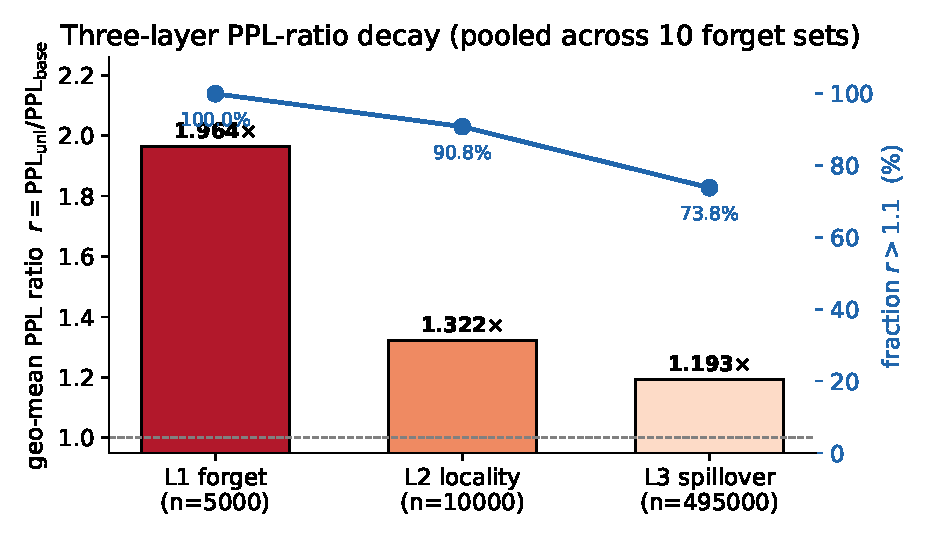
\includegraphics[width=0.95\columnwidth]{fig_three_layer_decay.pdf}
\caption{\textbf{Three-layer impact decay.} Left: geo-mean PPL ratio $r$ falls from $\Lforget{=}1.96\times$ to $\Lbyst{=}1.19\times$. Right: fraction of samples with $r{>}1.1$ ($100\%/90.8\%/73.8\%$). $\Lbyst$ bystander impact is non-zero in both senses.}
\label{fig:three-layer-decay}
\end{figure}

We also examine whether the profile is fixed by the algorithm, or whether it
depends on which forget set is chosen. Under identical optimisation, switching
$\Df$ changes the measured profile substantially: Table~\ref{tab:perforget}
contrasts the mildest and worst forget set among $100$, and
Fig.~\ref{fig:per-forget-profile} shows the full distribution.

\begin{table}[t]
\centering
\small
\setlength{\tabcolsep}{4pt}
\begin{tabular}{@{}lccc@{}}
    \toprule
                                                   & $\Lforget$ & $\Lneigh$ & $\Lbyst$ \\
    \midrule
    Mildest triplet (\texttt{029})                 & $1.54$ & $1.15$ & $1.12$ \\
    Worst triplet (\texttt{073}, ``storm'')        & $\mathbf{2.44}$ & $\mathbf{1.73}$ & $\mathbf{1.26}$ \\
    \midrule
    Spread (max/min, $n{=}100$)                    & $\mathbf{1.59\times}$ & $1.50\times$ & $1.13\times$ \\
    \bottomrule
\end{tabular}
\caption{Forget-set-induced variation. $\Lforget$ varies by $1.59\times$ between the mildest and worst $\Df$ under fixed algorithm/hyperparameters.}
\label{tab:perforget}
\end{table}

\begin{figure}[t]
\centering
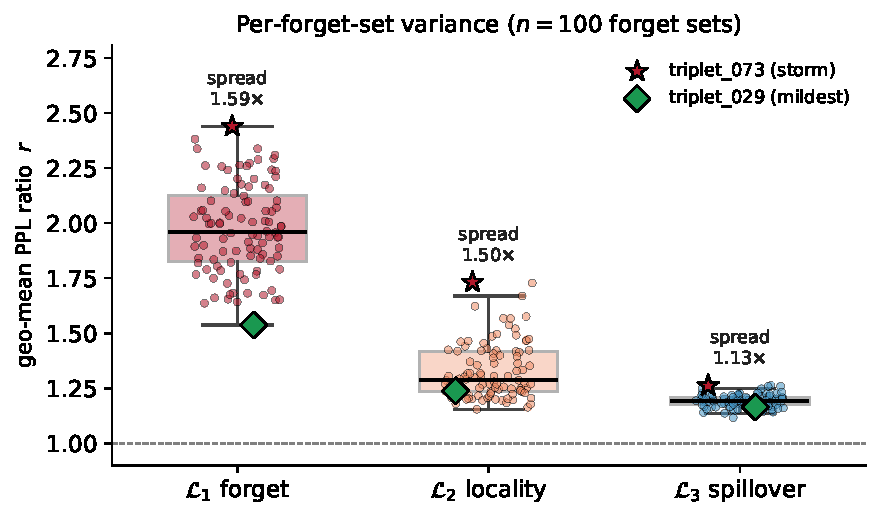
\includegraphics[width=0.95\columnwidth]{fig_per_forget_profile.pdf}
\caption{\textbf{Per-forget-set variance ($n{=}100$).} Box + jitter of geo-mean $r$ for each layer; one dot per forget set. Spread $\max/\min$ reaches $1.59\times$ on $\Lforget$, $1.50\times$ on $\Lneigh$, $1.13\times$ on $\Lbyst$. \texttt{triplet\_073} (``storm'') is the worst on $\Lforget$ and $\Lneigh$ but not on $\Lbyst$ (where \texttt{triplet\_072} is the maximum, $1.26\times$); \texttt{triplet\_029} is the $\Lforget$ minimum. Distribution shape is markedly tighter as the layer recedes from $\Df$.}
\label{fig:per-forget-profile}
\end{figure}

Together, these results support three observations.

\textbf{(C1) The three layers are strictly decreasing.}
The layer ordering is not an arbitrary binning choice: the measured impact
decreases monotonically from the forget set to neighbours to bystanders.
Table~\ref{tab:headline} gives
$\Lforget{=}1.96\times{>}\Lneigh{=}1.32\times{>}\Lbyst{=}1.19\times$, and
Fig.~\ref{fig:three-layer-decay} shows the same decay in both geo-mean PPL
ratio and the fraction of samples with $r{>}1.1$. The ordering also holds
within each cluster (Sec.~\ref{sec:invariants}), so it is not an artefact of
global aggregation.

\textbf{(C2) Bystander impact is not zero.}
The third layer is weaker than the first two, but cross-topic bystanders are
still measurably hit. $\Lbyst$ has geo-mean $1.19\times$, and $73.8\%$ of
cross-topic samples exceed $r{>}1.1$. These samples are not in the forget set
and are not same-topic neighbours of the unlearned triplet, so this is genuine
spillover rather than intended forgetting.

\textbf{(C3) The profile varies with the forget set.}
The same algorithm and hyperparameters do not produce a single fixed impact
profile. In Table~\ref{tab:perforget}, changing only $\Df$ moves $\Lforget$
from $1.54\times$ to $2.44\times$ and $\Lneigh$ from $1.15\times$ to
$1.73\times$; Fig.~\ref{fig:per-forget-profile} shows that this is a
distributional pattern rather than a single outlier. This variation makes the
forget set itself worth auditing before paying for full unlearning and
cross-evaluation.

% ============================================================================
% 5. Forget-Set Audit
% ============================================================================
\section{Forget-Set Audit}
\label{sec:audit}

Because the three-layer profile varies with $\Df$, forget-set choice becomes a
tunable design decision. The problem is that \emph{evaluating} that decision
currently requires running unlearning. We now ask whether $\Df$'s intrinsic
geometry is a sufficient signal to predict the three-layer impact profile
without ever fine-tuning.

\subsection{Audit Features}
\label{sec:features}

For each forget set $\Df$ of $50$ texts, we compute a $12$-dim intrinsic geometric descriptor from the same MiniLM embeddings used for clustering, with no access to model weights, gradients, or any unlearned checkpoint:
\begin{itemize}
    \setlength\itemsep{0.15em}
    \item \textbf{Spread (3)}: \texttt{emb\_variance\_mean}, \texttt{emb\_variance\_max}, \texttt{pairwise\_eucl\_mean}.
    \item \textbf{Similarity (3)}: \texttt{pairwise\_sim\_mean / std / q90} (cosine).
    \item \textbf{Location/scale (3)}: \texttt{centroid\_norm}, \texttt{emb\_norm\_mean / std}.
    \item \textbf{Shape (3)}: \texttt{effective\_rank}, \texttt{isotropy}, \texttt{spread\_over\_centroid}.
\end{itemize}
All $12$ features are scalars derived from the $50\times 384$ forget-set embedding matrix; computing them takes milliseconds per $\Df$.

\subsection{Audit Problem}
\label{sec:audit-problem}

\paragraph{Inputs.} The $50\!\times\!384$ embedding matrix of a candidate $\Df$, summarised by the $12$-dim geometric descriptor of Sec.~\ref{sec:features}. \emph{No} unlearned checkpoint, \emph{no} evaluation text, \emph{no} retain set is required.

\paragraph{Outputs.} Three scalars: predicted geo-mean $\log r$ for $\Lone$, $\Ltwo$, $\Lthree$. We treat audit primarily as a \emph{ranking} problem (which forget sets to flag by predicted impact), and report regression metrics for completeness.

\paragraph{Predictor.} Random Forest regression (\texttt{n\_estimators}{=}$200$, \texttt{min\_samples\_leaf}{=}$2$, \texttt{max\_depth}{=}\texttt{None}, \texttt{random\_state}{=}$0$), one regressor per layer, evaluated under leave-one-out (LOO over the $n{=}100$ forget sets; the held-out triplet never appears during fitting). The baseline predicts the mean of the $99$ training targets. Ridge / Lasso / Gradient Boosting baselines are reported in the ablation table (Sec.~\ref{sec:ablation}).

\subsection{Audit Performance}
\label{sec:audit-perf}

Table~\ref{tab:audit} reports held-out $R^2$, MAE, and Spearman $\rho$, plus $95\%$ percentile bootstrap CIs for $\rho$ ($n_{\text{boot}}{=}10{,}000$, seed $0$, bootstrapping over the $10$ LOO (true, predicted) cluster pairs).

\begin{table}[t]
\centering
\small
\setlength{\tabcolsep}{3.5pt}
\begin{tabular}{@{}lccc@{}}
    \toprule
                                  & $\Lone$            & $\Ltwo$            & $\Lthree$            \\
    \midrule
    Audit $R^2$                   & $\mathbf{+0.301}$  & $\mathbf{+0.735}$  & $\mathbf{+0.305}$    \\
    Baseline $R^2$ (LOO mean)     & $-0.020$           & $-0.020$           & $-0.020$             \\
    Audit MAE                     & $\mathbf{0.133}$   & $\mathbf{0.046}$   & $\mathbf{0.019}$     \\
    Baseline MAE                  & $0.169$            & $0.105$            & $0.022$              \\
    \midrule
    Spearman $\rho$               & $+0.560$           & $+0.869$           & $+0.592$             \\
    $\rho$ 95\% CI                & $[+0.40, +0.69]$   & $[+0.81, +0.91]$   & $[+0.44, +0.71]$     \\
    \bottomrule
\end{tabular}
\caption{Forget-set audit performance. LOO over $n{=}100$ forget sets; Random Forest ($n_{\text{est}}{=}200$, $\text{min\_leaf}{=}2$) on $12$-dim forget-set geometry. All three $\rho$ CIs exclude zero; $\Ltwo$ is the strongest layer, and $\Lthree$ CI is now strictly above zero.}
\label{tab:audit}
\end{table}

\begin{figure}[t]
\centering
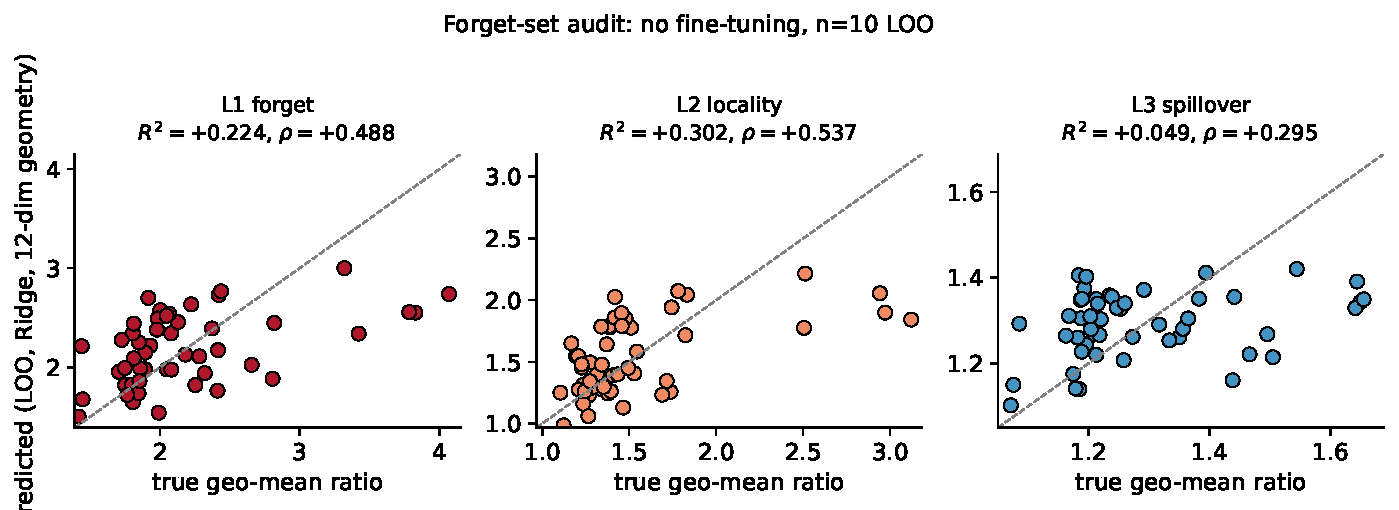
\includegraphics[width=0.95\columnwidth]{fig_audit_scatter.pdf}
\caption{\textbf{Audit scatter}, predicted vs.\ true geo-mean $\log r$. Each point is one held-out forget set under LOO. $\Ltwo$ is closest to the diagonal ($\rho{=}0.87$); $\Lone$ and $\Lthree$ are noisier but rank-significant ($\rho{=}0.56$, $0.59$).}
\label{fig:audit-scatter}
\end{figure}

\begin{figure}[t]
\centering
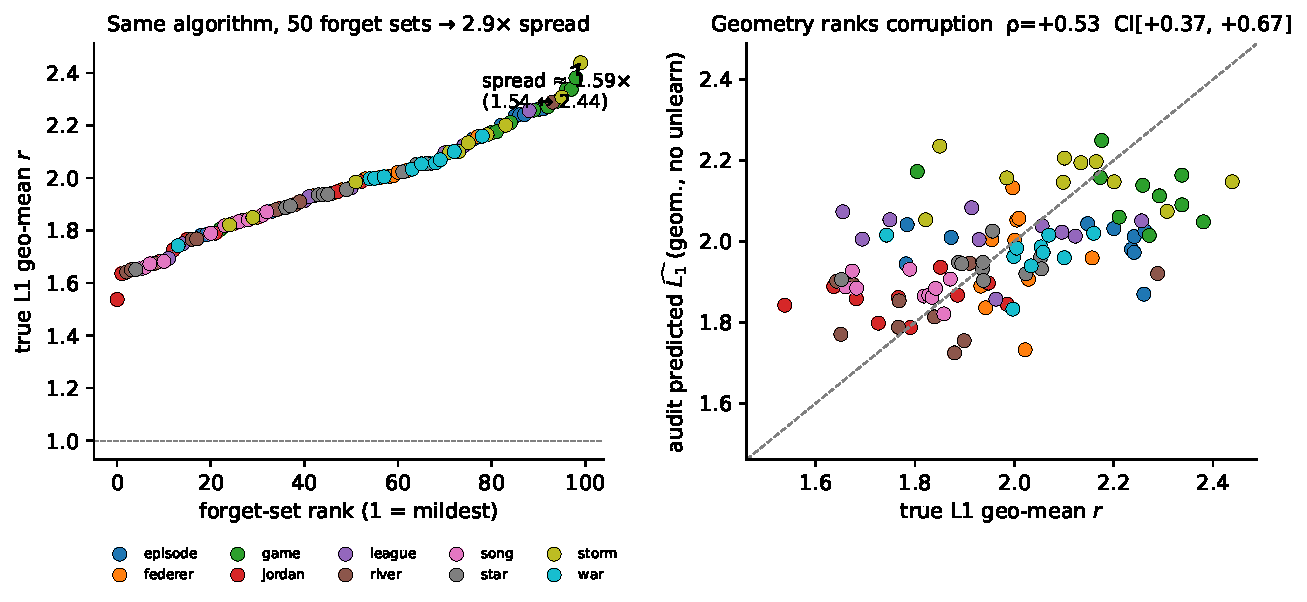
\includegraphics[width=0.95\columnwidth]{fig_forget_spread.pdf}
\caption{\textbf{Forget-set spread.} Distribution of per-forget-set $\Lone$ across the $100$ triplets, grouped by HDBSCAN cluster. The variation auditing must capture is between-cluster more than within-cluster.}
\label{fig:forget-spread}
\end{figure}

\textbf{$\Ltwo$ is the strongest layer.} With $R^2{=}0.74$ and $\rho{=}0.87$, the auditor recovers $74\%$ of locality variance from forget-set geometry alone --- consistent with the intuition that locality damage tracks how concentrated and self-similar $\Df$ is in embedding space.

\textbf{$\Lthree$ CI now excludes zero.} On a coarser problem ($n{=}10$ in early experiments) the L3 audit had $R^2{=}-0.46$; at $n{=}100$ the Random Forest auditor reaches $R^2{=}+0.30$ with $\rho{=}0.59$ ($95\%$ CI $[+0.44, +0.71]$). Statistical power and a non-linear model together close the previous gap; even the linear Ridge baseline (Sec.~\ref{sec:ablation}) reaches $\rho{=}0.49$ on the same $n{=}100$ slice.

\textbf{Audit cost.} Computing the $12$-dim feature for one $\Df$ takes milliseconds; fitting the Random Forest on $99$ training triplets is well under a second; predicting on a new $\Df$ is essentially instant. By contrast, evaluating one candidate $\Df$ via the standard pipeline costs one unlearn run ($\approx 75$\,s on H100) plus one column of cross-PPL ($\approx 220$\,s for $100$ eval pairs). At $n{=}100$ candidates the full grid is $\approx 7$ GPU-hours; the auditor runs in seconds on a CPU.

\subsection{Predictor Ablation}
\label{sec:ablation}

We compare the headline Random Forest auditor against three alternative
regressors on the same $12$-dim feature matrix and same LOO protocol
(Table~\ref{tab:ablation}): Ridge ($\alpha{=}1$, the simplest linear
baseline), Lasso ($\alpha{=}0.01$), and Gradient Boosting ($n_{\text{est}}{=}200$, $\text{depth}{=}3$, $\text{lr}{=}0.05$).

\begin{table}[t]
\centering
\small
\setlength{\tabcolsep}{3.5pt}
\begin{tabular}{@{}lccc@{}}
    \toprule
    Predictor                                 & $\Lone$            & $\Ltwo$            & $\Lthree$            \\
    \midrule
    \multicolumn{4}{@{}l@{}}{\textit{$R^2$ (LOO held-out)}} \\
    Random Forest (headline)                  & $\mathbf{+0.301}$  & $\mathbf{+0.735}$  & $\mathbf{+0.305}$    \\
    Gradient Boosting                         & $+0.209$           & $+0.743$           & $+0.200$             \\
    Ridge ($\alpha{=}1$)                      & $+0.246$           & $+0.705$           & $+0.215$             \\
    Lasso ($\alpha{=}0.01$)                   & $+0.224$           & $+0.644$           & $+0.088$             \\
    \midrule
    \multicolumn{4}{@{}l@{}}{\textit{Spearman $\rho$}} \\
    Random Forest (headline)                  & $\mathbf{+0.560}$  & $\mathbf{+0.869}$  & $\mathbf{+0.592}$    \\
    Gradient Boosting                         & $+0.524$           & $+0.879$           & $+0.534$             \\
    Ridge ($\alpha{=}1$)                      & $+0.531$           & $+0.840$           & $+0.491$             \\
    Lasso ($\alpha{=}0.01$)                   & $+0.494$           & $+0.849$           & $+0.380$             \\
    \bottomrule
\end{tabular}
\caption{Predictor ablation on the same $12$-dim feature matrix and LOO protocol ($n{=}100$). RF and GB are the strongest non-linear models and tie on $\Ltwo$; the linear Ridge baseline already lifts all three layers above the LOO-mean baseline ($R^2{=}{-}0.02$). Lasso under-fits on $\Lthree$ (sparse solution discards most features). Choosing the non-linear ceiling matters most for $\Lthree$, where RF gains $+0.09$ in $R^2$ over Ridge.}
\label{tab:ablation}
\end{table}

The non-linear models (RF, GB) tie on the strongest layer ($\Ltwo$), but RF
edges out on $\Lone$ and $\Lthree$ where forget-set geometry interactions
appear to matter more. The linear Ridge baseline ($\rho{=}0.49$ on $\Lthree$
with CI $[+0.33, +0.63]$, also strictly above zero) already gives a
deployable pre-screen, indicating that a substantial fraction of the
audit signal is linear in the geometric descriptor.

\subsection{Unlearner Generality (NPO)}
\label{sec:cross-unlearner}

To probe whether the audit framework is bound to GradAscent, we replicate the
full pipeline with NPO \citep{zhang2024negative}: a different unlearning
algorithm with the same TOFU-aligned hyperparameters on the same $n{=}100$
forget sets, yielding a parallel $100\times100$ cross-PPL grid and the same
$12$-dim geometric descriptor as input. The audit predictor (Random Forest,
identical hyperparameters and LOO protocol) is trained and evaluated
independently on NPO labels — we do not transfer predictions across unlearners.

\begin{table}[t]
\centering
\small
\setlength{\tabcolsep}{3pt}
\begin{tabular}{@{}llccc@{}}
    \toprule
    & & $\Lforget$ & $\Lneigh$ & $\Lbyst$ \\
    \midrule
    \multirow{2}{*}{\textit{Headline geo $r$}}
       & GradAscent & $1.96\times$       & $1.32\times$       & $1.19\times$       \\
       & NPO        & $1.68\times$       & $1.15\times$       & $1.11\times$       \\
    \midrule
    \multirow{2}{*}{\textit{Audit $\rho$}}
       & GradAscent & $+0.560$           & $\mathbf{+0.869}$  & $+0.592$           \\
       & NPO        & $\mathbf{+0.657}$  & $+0.823$           & $+0.506$           \\
    \midrule
    \multirow{2}{*}{\textit{$\rho$ 95\% CI}}
       & GradAscent & $[+0.40,+0.69]$    & $[+0.81,+0.91]$    & $[+0.44,+0.71]$    \\
       & NPO        & $[+0.52,+0.76]$    & $[+0.72,+0.89]$    & $[+0.34,+0.65]$    \\
    \midrule
    \multirow{2}{*}{\textit{top-10\% recall}}
       & GradAscent & $2/10$             & $6/10$             & $3/10$             \\
       & NPO        & $2/10$             & $\mathbf{8/10}$    & $\mathbf{5/10}$    \\
    \bottomrule
\end{tabular}
\caption{Cross-unlearner audit. Same $12$-dim geometric features, same RF protocol, same LOO over $n{=}100$ forget sets — only the unlearning algorithm changes. NPO produces ${\sim}10\text{--}14\%$ milder per-layer impact than GradAscent, but the audit recovers rank-significant predictions on both, with all six $\rho$ CIs strictly above zero.}
\label{tab:cross-unlearner}
\end{table}

\textbf{Take-away.} The audit predictor is unlearner-agnostic: the $12$-dim
forget-set descriptor lifts all three layers above the LOO-mean baseline for
both GradAscent and NPO under independent training. Top-10\% recall is in fact
higher on NPO ($8/10$ on $\Lneigh$, $5/10$ on $\Lbyst$), likely because NPO's
narrower dynamic range makes the ranking task easier. The same conclusion is
reached separately per unlearner without label transfer between them.

\subsection{Positioning: a Pre-Screen, Not a Replacement}
\label{sec:positioning}

We position the auditor as a \emph{warning tool} for the forget-set selection step, not as a substitute for the actual unlearning evaluation.

\begin{table}[t]
\centering
\small
\setlength{\tabcolsep}{3pt}
\renewcommand{\arraystretch}{1.05}
\begin{tabular}{@{}p{0.18\columnwidth} p{0.36\columnwidth} p{0.36\columnwidth}@{}}
    \toprule
              & \textbf{Can}                                  & \textbf{Cannot} \\
    \midrule
    Rank      & flag ``which $\Df$ is worse'' ($\rho$ CIs $\!>\!0$, $\Ltwo$ $0.87$) & assign trustworthy absolute PPL values \\
    Screen    & red/yellow/green warnings on candidates       & score an unlearning algorithm \\
    Compute   & seconds vs.\ several GPU-hours                & replace the final unlearn run \\
    \bottomrule
\end{tabular}
\caption{Audit positioning: cheap pre-screen for forget-set selection.}
\label{tab:positioning}
\end{table}

\paragraph{Workflow.} Given $N$ candidate forget sets, audit all $N$ in seconds, sort by predicted impact profile, and run real unlearning only on the top-$k$. At $N{=}100$ and $k{=}10$, the pre-screen reduces the unlearning budget by $10\times$ while retaining the worst-case offenders identified by the auditor.

% ============================================================================
% 6. Discussion
% ============================================================================
\section{Discussion}
\label{sec:discussion}

\subsection{What the geometric features actually capture}
\label{sec:why-it-works}

A natural question is why $12$ scalar features computed in milliseconds carry enough signal to rank the locality damage with $\rho{=}0.87$. We hypothesise three mechanisms, each consistent with the per-cluster pattern in Fig.~\ref{fig:per-forget-profile}:
\begin{itemize}
    \setlength\itemsep{0.15em}
    \item \textbf{Concentration $\Rightarrow$ stronger locality damage}. Forget sets with low spread and high pairwise similarity (e.g.\ the ``storm'' cluster) sit on a tight manifold; the gradient signal from GradAscent is therefore sharply directional, and validation/test neighbours along the same direction are dragged with it. This predicts large $\Ltwo$, which we observe.
    \item \textbf{Effective rank $\Rightarrow$ spillover footprint}. Low-effective-rank $\Df$ lives near a low-dim subspace; updating the model along that subspace bleeds across topic clusters that share the same dominant directions, producing $\Lthree{>}1$. The (negative) correlation between subspace coverage and $\Lthree$ ($\rho{=}{-}0.48$) supports this view.
    \item \textbf{Centroid norm $\Rightarrow$ baseline PPL coupling}. Forget sets far from the embedding origin tend to have higher base PPL, which inflates the $r{=}\PPL_{\text{unlearned}}/\PPL_{\text{base}}$ ratio's denominator unevenly across layers; capturing this with \texttt{centroid\_norm} corrects for the floor.
\end{itemize}
A causal study --- e.g.\ deliberately constructing $\Df$ with prescribed isotropy and effective rank --- is left to future work; the present paper establishes the predictive correlation under naturally occurring HDBSCAN clusters.

\subsection{When does the auditor break?}
\label{sec:failure}

The audit is most reliable for $\Ltwo$ and least reliable for $\Lthree$ in absolute terms (RF MAE $0.019$ vs.\ baseline $0.022$ --- a $14\%$ improvement, with $\rho{=}0.59$ and $95\%$ CI $[+0.44, +0.71]$). Two reasons: (i) $\Lthree$ has a very narrow dynamic range ($1.13\times$ between worst and mildest cluster), so absolute prediction is intrinsically hard; and (ii) cross-cluster spillover plausibly depends on \emph{evaluation-side} geometry (where the neighbours of $\Df$ are in the broader embedding space), which the forget-set-only descriptor cannot see. Top-1 identification is unstable in the same-cluster regime (multiple triplets within a cluster have very similar predicted scores), which is why we frame the auditor as a top-$k$ screen rather than a precise ranker.

\subsection{Limitations}
\label{sec:limitations}

We acknowledge three ``singles'' that the present study does not control for:
\begin{enumerate}
    \setlength\itemsep{0.15em}
    \item \textbf{Single base model} (Llama-3.1-8B-Instruct). Geometry-to-corruption mapping may be model-specific; verifying on Mistral-7B and a Qwen variant is high-priority next work.
    \item \textbf{$n{=}100$}. All three CIs exclude zero on both unlearners (Sec.~\ref{sec:cross-unlearner}), but $\Lbyst$ remains the weakest layer; scaling to $n{=}500$--$1000$ is feasible in one extra GPU-day.
    \item \textbf{Single metric}: PPL ratio. PPL captures token-level corruption but not task-level utility (QA accuracy). Parallel QA-based evaluation is in progress as a complementary axis.
\end{enumerate}
GradDiff and RMU are the natural next unlearners to add (alongside the GradAscent + NPO pair already covered).

\subsection{Ethical and Practical Considerations}
\label{sec:ethics}

A pre-screen that ranks forget sets by side-effect could in principle be misused to \emph{target} forget sets that maximise damage (e.g.\ to degrade a competitor's model via a poisoned removal request). We see two mitigations: (i) the auditor itself is not a generative tool --- it scores, not produces, candidates; (ii) the failure mode is bounded by the underlying unlearning algorithm, which already has well-known damage profiles independent of our score. We recommend that practical deployments couple the auditor with a downstream gate (the actual unlearn + cross-PPL), as in the screen-then-run workflow of Sec.~\ref{sec:positioning}.

% ============================================================================
% 7. Conclusion
% ============================================================================
\section{Conclusion}
\label{sec:conclusion}

We characterised LLM unlearning side-effects on Llama-3.1-8B-Instruct across $n{=}100$ forget sets and $1.5$M per-sample evaluations, and re-cast the resulting benchmarking burden as a forget-set audit problem.

\paragraph{Findings.} (i) Side-effects decay monotonically across three semantic layers ($\Lone{=}1.96\times$, $\Ltwo{=}1.32\times$, $\Lthree{=}1.19\times$) but $\Lthree$ never reaches zero --- $73.8\%$ of cross-topic samples are still corrupted. (ii) Under fixed algorithm and hyperparameters, $\Lone$ varies $1.59\times$ between the mildest and worst forget set, identifying $\Df$ itself as a substantial source of variation. (iii) A Random Forest regressor on $12$-dim forget-set geometry predicts the layer profile with leave-one-out Spearman $\rho$ of $0.56/0.87/0.59$, all $95\%$ CIs strictly above zero. (iv) The same audit pipeline applied to NPO yields independent rank-significant predictions ($\rho{=}0.66/0.82/0.51$), confirming the methodology is unlearner-agnostic.

\paragraph{Implication.} Unlearning evaluation can adopt a \emph{screen-then-run} workflow: rank candidate forget sets by audit score, run real unlearning only on the top-$k$. At $N{=}100$, $k{=}10$, this trades $7$ GPU-hours of cross-PPL for seconds of CPU --- without renouncing the ground-truth check on whatever the auditor flags.

\paragraph{Future work.} Cross-unlearner transfer (NPO, GradDiff, RMU), cross-model audit (Mistral-7B, Qwen), enriching the descriptor with mutual-reachability and signed projection coverage, scaling to $n{=}500$--$1000$, and parallel QA-accuracy metrics for non-PPL utility. We release the cross-PPL matrix, audit features, and pre-screen code to enable these extensions.

% ============================================================================
% 8. Related Work
% ============================================================================
\section{Related Work}
\label{sec:related}

\paragraph{LLM unlearning algorithms and benchmarks.}
Modern LLM unlearning uses gradient-based or preference-based fine-tuning to push the model to forget targeted data while preserving the rest. Representative algorithms include \emph{Gradient Ascent} (GradAscent) and gradient-difference variants \citep{jang2023knowledge}, \emph{NPO} (Negative Preference Optimisation) \citep{zhang2024negative}, and \emph{representation misdirection} \citep{li2024wmdp}. Benchmarks such as TOFU \citep{maini2024tofu}, MUSE \citep{shi2024muse}, and WMDP \citep{li2024wmdp} fix specific forget splits and report aggregate forget-quality and utility scores. The unifying \emph{OpenUnlearning} framework \citep{dorna2025openunlearning} integrates $13$ algorithms and $16$ metrics under one Hydra-configured trainer; we vendor it as our stage-2 implementation. These works concentrate on \emph{algorithm choice} given a benchmark forget split. Our work is orthogonal: we hold the algorithm and hyperparameters fixed and study how the choice of $\Df$ itself reshapes the three-layer impact profile, then turn the observation into a pre-screen for $\Df$.

\paragraph{Side-effects, locality, and knowledge holes.}
Unlearning is increasingly recognised as collateral-damaging. \citet{ko2025probing} introduce \emph{knowledge-hole probing}: standard utility benchmarks miss adjacent and latent knowledge that has been silently damaged by unlearning, and dedicated probes can recover this damage post-hoc. Studies of model editing \citep{meng2022locating, mitchell2022memory} and influence functions \citep{koh2017understanding, grosse2023studying} show analogous locality / non-locality effects in the gradient-update regime. Our three-layer view operationalises Ko et al.'s phenomenon as a quantitative, dataset-driven measurement: $\Ltwo$ corresponds to their \emph{adjacent} knowledge (same-cluster neighbours), and $\Lthree$ extends the picture to \emph{cross-cluster spillover} that prior probes did not target. Crucially, while their probes act \emph{after} unlearning, our audit acts \emph{before} --- predicting the impact profile from $\Df$ alone.

\paragraph{Data-first prediction of model behaviour.}
A separate line of work predicts downstream model behaviour from properties of the training data, rather than from running the model. \citet{dang2024curious} predict the adversarial robustness of fine-tuned text transformers from features of the fine-tuning dataset, achieving $30\!\times\!\text{--}\!193\times$ acceleration over the standard model-first attack-then-evaluate pipeline. Related efforts use coreset and data-attribution descriptors \citep{koh2017understanding, ilyas2022datamodels}, dataset diversity statistics \citep{wang2024data}, and curvature of the loss landscape \citep{yao2020pyhessian} to predict generalisation or vulnerability. We carry this paradigm into LLM unlearning: instead of running unlearning and then measuring its impact profile, we measure intrinsic geometry of $\Df$ and predict that profile directly. To our knowledge, this is the first \emph{data-first} predictor in the unlearning setting.

\paragraph{Forget-set selection and curation.}
A small body of work studies which data is hardest to remove or causes the most damage when removed \citep{thudi2022unrolling, kurmanji2024towards}. The closest setting is influence-based forget-set selection \citep{koh2017understanding}, but influence functions require gradients of the trained model, scale poorly to $8$B-parameter LLMs, and yield a per-example score rather than a $\Df$-level impact profile. Our auditor uses only $50$ forget-set embeddings and $12$ scalar features; it is two orders of magnitude cheaper and produces a three-layer profile.

\paragraph{Position.}
We sit at the intersection of unlearning impact characterisation \citep{ko2025probing} and data-first behaviour prediction \citep{dang2024curious}. The first tells us \emph{what to predict} (intended degradation + locality damage + spillover damage); the second tells us \emph{how to predict from data alone}. Our contribution is the quantitative bridge: a three-layer impact metric tied to a forget-set-side geometric audit.

\bibliography{references}

\appendix
% ============================================================================
% A. Reproducibility Details + Additional Sanity Tables
% ============================================================================
\section{Reproducibility Details}
\label{app:repro}

\paragraph{Data preparation.} WikiText-103 is filtered to $16{,}038$ passages of length $\geq 32$ tokens; embeddings come from \texttt{all-MiniLM-L6-v2} (no dimensionality reduction; the first $384$ dims are taken as-is). HDBSCAN parameters: \texttt{min\_cluster\_size}{=}$200$, \texttt{min\_samples}{=}$5$, Euclidean metric, EOM cluster selection. The resulting cluster-size distribution is $202 / 346 / 3{,}276$ (min/median/max). $100$ triplets are sampled with seed $42$, requiring \texttt{required\_cluster\_size}{=}$150$ and $50$ texts per split; per-triplet splits are guaranteed disjoint within a triplet.

\paragraph{Unlearning hyperparameters.} GradAscent in OpenUnlearning's \texttt{wikitext\_unlearn\_tofu\_aligned.sh}: \texttt{num\_train\_epochs}{=}$5$, \texttt{per\_device\_train\_batch\_size}{=}$8$, \texttt{gradient\_accumulation\_steps}{=}$8$ (effective batch $64$), \texttt{learning\_rate}{=}$1\!\times\!10^{-5}$ with linear schedule to zero, \texttt{warmup\_steps}{=}$1$, \texttt{weight\_decay}{=}$0.01$, \texttt{paged\_adamw\_32bit}, BF16. With $|\Df|{=}50$ and effective batch $64$, exactly $5$ optimiser steps fire (one per epoch); train-loss range $[-0.84, -0.62]$.

\paragraph{Evaluation.} PPL is computed in BF16 with stride $512$ and context $1024$; each text is scored independently. Base-model PPL is cached once per (eval triplet, split) and re-used across the $100$ unlearned checkpoints. Long-format output: \texttt{ppl\_long.parquet} with one row per $(m, e, s, i)$.

\paragraph{Audit feature scripts.} \texttt{features/forget\_set.py} computes the $12$ scalars from a $50\!\times\!384$ embedding matrix in $<\!10$\,ms. Random Forest regression: \texttt{sklearn.ensemble.RandomForestRegressor} with \texttt{n\_estimators}{=}$200$, \texttt{min\_samples\_leaf}{=}$2$, \texttt{max\_depth}{=}\texttt{None}, \texttt{random\_state}{=}$0$, leave-one-out grouping over $n{=}100$ forget sets. Bootstrap: $10{,}000$ resamples of the $100$ LOO (true, predicted) pairs with seed $0$.

\paragraph{Hardware.} All runs on a single H100 (80\,GB) node. End-to-end wall-clock: data prep $\approx 20$ min; $100$ unlearn runs $1$\,h\,$54$\,min; cross-PPL $6$\,h\,$11$\,min.

\section{Additional Sanity Tables}
\label{app:tables}

\paragraph{Per-cluster monotonicity.} Across all $10$ clusters, $\Lone(c){>}\Ltwo(c){>}\Lthree(c)$ holds without exception; the smallest within-cluster gap $\Lone{-}\Ltwo$ is $0.39$ (mildest cluster) and the largest is $0.71$ (storm). Per-cluster table is included in \texttt{corruption\_summary.json}.

\paragraph{Coverage diagnostic.} The Pearson correlation between forget-set ball-coverage and $\Lthree$ is $r{=}{-}0.16$ (Spearman $\rho{=}{-}0.48$); a higher coverage of the embedding space corresponds to lower spillover, consistent with the rank-based mechanism in Sec.~\ref{sec:why-it-works}. Replacing ball coverage with a signed-projection or mutual-reachability variant is left for future work.

\end{document}
